


\documentclass[conference]{IEEEtran}
% Some Computer Society conferences also require the compsoc mode option,
% but others use the standard conference format.
%
% If IEEEtran.cls has not been installed into the LaTeX system files,
% manually specify the path to it like:
% \documentclass[conference]{../sty/IEEEtran}





% Some very useful LaTeX packages include:
% (uncomment the ones you want to load)


% *** MISC UTILITY PACKAGES ***
%
%\usepackage{ifpdf}
% Heiko Oberdiek's ifpdf.sty is very useful if you need conditional
% compilation based on whether the output is pdf or dvi.
% usage:
% \ifpdf
%   % pdf code
% \else
%   % dvi code
% \fi
% The latest version of ifpdf.sty can be obtained from:
% http://www.ctan.org/pkg/ifpdf
% Also, note that IEEEtran.cls V1.7 and later provides a builtin
% \ifCLASSINFOpdf conditional that works the same way.
% When switching from latex to pdflatex and vice-versa, the compiler may
% have to be run twice to clear warning/error messages.






% *** CITATION PACKAGES ***
%
\usepackage{cite}
% cite.sty was written by Donald Arseneau
% V1.6 and later of IEEEtran pre-defines the format of the cite.sty package
% \cite{} output to follow that of the IEEE. Loading the cite package will
% result in citation numbers being automatically sorted and properly
% "compressed/ranged". e.g., [1], [9], [2], [7], [5], [6] without using
% cite.sty will become [1], [2], [5]--[7], [9] using cite.sty. cite.sty's
% \cite will automatically add leading space, if needed. Use cite.sty's
% noadjust option (cite.sty V3.8 and later) if you want to turn this off
% such as if a citation ever needs to be enclosed in parenthesis.
% cite.sty is already installed on most LaTeX systems. Be sure and use
% version 5.0 (2009-03-20) and later if using hyperref.sty.
% The latest version can be obtained at:
% http://www.ctan.org/pkg/cite
% The documentation is contained in the cite.sty file itself.






% *** GRAPHICS RELATED PACKAGES ***
%
\ifCLASSINFOpdf
  % \usepackage[pdftex]{graphicx}
  % declare the path(s) where your graphic files are
  % \graphicspath{{../pdf/}{../jpeg/}}
  % and their extensions so you won't have to specify these with
  % every instance of \includegraphics
  % \DeclareGraphicsExtensions{.pdf,.jpeg,.png}
\else
  % or other class option (dvipsone, dvipdf, if not using dvips). graphicx
  % will default to the driver specified in the system graphics.cfg if no
  % driver is specified.
  % \usepackage[dvips]{graphicx}
  % declare the path(s) where your graphic files are
  % \graphicspath{{../eps/}}
  % and their extensions so you won't have to specify these with
  % every instance of \includegraphics
  % \DeclareGraphicsExtensions{.eps}
\fi
% graphicx was written by David Carlisle and Sebastian Rahtz. It is
% required if you want graphics, photos, etc. graphicx.sty is already
% installed on most LaTeX systems. The latest version and documentation
% can be obtained at: 
% http://www.ctan.org/pkg/graphicx
% Another good source of documentation is "Using Imported Graphics in
% LaTeX2e" by Keith Reckdahl which can be found at:
% http://www.ctan.org/pkg/epslatex
%
% latex, and pdflatex in dvi mode, support graphics in encapsulated
% postscript (.eps) format. pdflatex in pdf mode supports graphics
% in .pdf, .jpeg, .png and .mps (metapost) formats. Users should ensure
% that all non-photo figures use a vector format (.eps, .pdf, .mps) and
% not a bitmapped formats (.jpeg, .png). The IEEE frowns on bitmapped formats
% which can result in "jaggedy"/blurry rendering of lines and letters as
% well as large increases in file sizes.
%
% You can find documentation about the pdfTeX application at:
% http://www.tug.org/applications/pdftex





% *** MATH PACKAGES ***
%
\usepackage{amsmath}
% A popular package from the American Mathematical Society that provides
% many useful and powerful commands for dealing with mathematics.
%
% Note that the amsmath package sets \interdisplaylinepenalty to 10000
% thus preventing page breaks from occurring within multiline equations. Use:
%\interdisplaylinepenalty=2500
% after loading amsmath to restore such page breaks as IEEEtran.cls normally
% does. amsmath.sty is already installed on most LaTeX systems. The latest
% version and documentation can be obtained at:
% http://www.ctan.org/pkg/amsmath





% *** SPECIALIZED LIST PACKAGES ***
%
%\usepackage{algorithmic}
% algorithmic.sty was written by Peter Williams and Rogerio Brito.
% This package provides an algorithmic environment fo describing algorithms.
% You can use the algorithmic environment in-text or within a figure
% environment to provide for a floating algorithm. Do NOT use the algorithm
% floating environment provided by algorithm.sty (by the same authors) or
% algorithm2e.sty (by Christophe Fiorio) as the IEEE does not use dedicated
% algorithm float types and packages that provide these will not provide
% correct IEEE style captions. The latest version and documentation of
% algorithmic.sty can be obtained at:
% http://www.ctan.org/pkg/algorithms
% Also of interest may be the (relatively newer and more customizable)
% algorithmicx.sty package by Szasz Janos:
% http://www.ctan.org/pkg/algorithmicx




% *** ALIGNMENT PACKAGES ***
%
%\usepackage{array}
% Frank Mittelbach's and David Carlisle's array.sty patches and improves
% the standard LaTeX2e array and tabular environments to provide better
% appearance and additional user controls. As the default LaTeX2e table
% generation code is lacking to the point of almost being broken with
% respect to the quality of the end results, all users are strongly
% advised to use an enhanced (at the very least that provided by array.sty)
% set of table tools. array.sty is already installed on most systems. The
% latest version and documentation can be obtained at:
% http://www.ctan.org/pkg/array


% IEEEtran contains the IEEEeqnarray family of commands that can be used to
% generate multiline equations as well as matrices, tables, etc., of high
% quality.




% *** SUBFIGURE PACKAGES ***
%\ifCLASSOPTIONcompsoc
%  \usepackage[caption=false,font=normalsize,labelfont=sf,textfont=sf]{subfig}
%\else
%  \usepackage[caption=false,font=footnotesize]{subfig}
%\fi
% subfig.sty, written by Steven Douglas Cochran, is the modern replacement
% for subfigure.sty, the latter of which is no longer maintained and is
% incompatible with some LaTeX packages including fixltx2e. However,
% subfig.sty requires and automatically loads Axel Sommerfeldt's caption.sty
% which will override IEEEtran.cls' handling of captions and this will result
% in non-IEEE style figure/table captions. To prevent this problem, be sure
% and invoke subfig.sty's "caption=false" package option (available since
% subfig.sty version 1.3, 2005/06/28) as this is will preserve IEEEtran.cls
% handling of captions.
% Note that the Computer Society format requires a larger sans serif font
% than the serif footnote size font used in traditional IEEE formatting
% and thus the need to invoke different subfig.sty package options depending
% on whether compsoc mode has been enabled.
%
% The latest version and documentation of subfig.sty can be obtained at:
% http://www.ctan.org/pkg/subfig




% *** FLOAT PACKAGES ***
%
%\usepackage{fixltx2e}
% fixltx2e, the successor to the earlier fix2col.sty, was written by
% Frank Mittelbach and David Carlisle. This package corrects a few problems
% in the LaTeX2e kernel, the most notable of which is that in current
% LaTeX2e releases, the ordering of single and double column floats is not
% guaranteed to be preserved. Thus, an unpatched LaTeX2e can allow a
% single column figure to be placed prior to an earlier double column
% figure.
% Be aware that LaTeX2e kernels dated 2015 and later have fixltx2e.sty's
% corrections already built into the system in which case a warning will
% be issued if an attempt is made to load fixltx2e.sty as it is no longer
% needed.
% The latest version and documentation can be found at:
% http://www.ctan.org/pkg/fixltx2e


%\usepackage{stfloats}
% stfloats.sty was written by Sigitas Tolusis. This package gives LaTeX2e
% the ability to do double column floats at the bottom of the page as well
% as the top. (e.g., "\begin{figure*}[!b]" is not normally possible in
% LaTeX2e). It also provides a command:
%\fnbelowfloat
% to enable the placement of footnotes below bottom floats (the standard
% LaTeX2e kernel puts them above bottom floats). This is an invasive package
% which rewrites many portions of the LaTeX2e float routines. It may not work
% with other packages that modify the LaTeX2e float routines. The latest
% version and documentation can be obtained at:
% http://www.ctan.org/pkg/stfloats
% Do not use the stfloats baselinefloat ability as the IEEE does not allow
% \baselineskip to stretch. Authors submitting work to the IEEE should note
% that the IEEE rarely uses double column equations and that authors should try
% to avoid such use. Do not be tempted to use the cuted.sty or midfloat.sty
% packages (also by Sigitas Tolusis) as the IEEE does not format its papers in
% such ways.
% Do not attempt to use stfloats with fixltx2e as they are incompatible.
% Instead, use Morten Hogholm'a dblfloatfix which combines the features
% of both fixltx2e and stfloats:
%
% \usepackage{dblfloatfix}
% The latest version can be found at:
% http://www.ctan.org/pkg/dblfloatfix




% *** PDF, URL AND HYPERLINK PACKAGES ***
%
%\usepackage{url}
% url.sty was written by Donald Arseneau. It provides better support for
% handling and breaking URLs. url.sty is already installed on most LaTeX
% systems. The latest version and documentation can be obtained at:
% http://www.ctan.org/pkg/url
% Basically, \url{my_url_here}.





% *** Do not adjust lengths that control margins, column widths, etc. ***
% *** Do not use packages that alter fonts (such as pslatex).         ***
% There should be no need to do such things with IEEEtran.cls V1.6 and later.
% (Unless specifically asked to do so by the journal or conference you plan
% to submit to, of course. )


% correct bad hyphenation here
\hyphenation{op-tical net-works semi-conduc-tor}


\usepackage{pgfplots}
\pgfplotsset{compat=1.7}
\usepackage{pgfplotstable}
\pgfplotstableset{col sep=comma}
\newcommand{\APW}{\textit{APW}}
\newcommand{\VPW}{\textit{VPW}}
\newcommand{\APH}{\textit{APH}}
\newcommand{\VPH}{\textit{VPH}}
\DeclareMathOperator{\sgn}{sign}
\DeclareMathOperator*{\argmin}{arg\,min}

\begin{document}
%
% paper title
% Titles are generally capitalized except for words such as a, an, and, as,
% at, but, by, for, in, nor, of, on, or, the, to and up, which are usually
% not capitalized unless they are the first or last word of the title.
% Linebreaks \\ can be used within to get better formatting as desired.
% Do not put math or special symbols in the title.
\title{Real-Time, Nonparametric Algorithm to Learn
Parameters for Pacemaker Beat Detection}


% author names and affiliations
% use a multiple column layout for up to three different
% affiliations
\author{\IEEEauthorblockN{Yamin Arefeen\IEEEauthorrefmark{1}, Daniel Zdeblick\IEEEauthorrefmark{1}, Philip Taffet\IEEEauthorrefmark{2}, Jorge Quintero\IEEEauthorrefmark{1}, Greg Harper\IEEEauthorrefmark{1},\\
Benhaam Aazhang\IEEEauthorrefmark{1}, and Joseph Cavallaro\IEEEauthorrefmark{1}}
\IEEEauthorblockA{\IEEEauthorrefmark{1}Department of Electrical and Computer Engineering, \IEEEauthorrefmark{2}Department of Computer Science\\
	Rice University, Houston, TX 77005}
	\IEEEauthorblockA{yarefeen@mit.edu, zdeblick@uw.edu, ptaffet@rice.edu, aaz@rice.edu, cavallar@rice.edu}
}

% conference papers do not typically use \thanks and this command
% is locked out in conference mode. If really needed, such as for
% the acknowledgment of grants, issue a \IEEEoverridecommandlockouts
% after \documentclass


% use for special paper notices
%\IEEEspecialpapernotice{(Invited Paper)}




% make the title area
\maketitle

% As a general rule, do not put math, special symbols or citations
% in the abstract
\begin{abstract}
While beat detection in a Cardiac Electrical 
Signal (CES) is a well-studied problem, we propose a novel
algorithm, within the context of pacemakers, that learns the
heights and widths of atrial and ventricular peaks from simply
processing 10 seconds of cardiac data sampled at 1 kHz. Utilizing
a purely data-driven solution to learn the parameters of atrial
and ventricular peaks will allow pacemakers to set their own
detection parameters for a specific patient and adaptively tune
their detection parameters over time for that specific patient.
We have validated these results on 51 separate channels of CES
data. Additionally, we have implemented the algorithm on a
Field Programmable Gate Array and tested it on an ex-vivo rat
heart to illustrate that our algorithm can be implemented on
hardware and run in real time.
\end{abstract}

% no keywords




% For peer review papers, you can put extra information on the cover
% page as needed:
% \ifCLASSOPTIONpeerreview
% \begin{center} \bfseries EDICS Category: 3-BBND \end{center}
% \fi
%
% For peerreview papers, this IEEEtran command inserts a page break and
% creates the second title. It will be ignored for other modes.
\IEEEpeerreviewmaketitle



\section{Introduction}
% no \IEEEPARstart
Cardiac diseases are the most common cause of death in
the United States. More than 600,000 people each year
die due to some failure in the heart~\cite{death-stats}. A healthy heart
functions through a regular cardiac cycle, where the pacemaking cells
in the sinoatrial (SA) node of the heart
generate an electrical signal, which travels from the atria
down to the ventricles, to stimulate heart contraction.
Many heart failures result from the heart's inability to
generate or conduct these electrical signals and stimulate
muscle contraction properly.

To combat this, doctors implant artificial electronic pacemakers
that can stimulate the heart
to contract artificially through externally supplied
electrical pulses.
Current pacemakers use the state of the art
algorithm called DDDR in order to determine whether
the heart requires stimulation~\cite{basic-pacing}.
The devices implement
CES beat detection algorithms to determine whether a
heartbeat has occurred. If the pacemaker does not detect a heartbeat
within a certain period of time, it will deliver an
electrical stimulation to the heart.

CES beat detection itself is a well-studied problem, as
several algorithms have been proposed to identify the
beats within an CES ~\cite{realtime-qrs, ecg-filter}. However, current
algorithms perform beat detection without distinguishing
which part of the CES corresponds to the atrial
portion of the heartbeat and which part corresponds to
the ventricular portion of the heartbeat. As a result,
current pacemakers often times struggle to distinguish
between atrial and ventricular beats: information that is
crucial for Cardiac Resynchronization Therapy (CRT)~\cite{multisite-crt}.
In fact, up to 30\% of patients with pacemakers do
not respond to CRT implemented by current pacemakers~\cite{multisite-crt}.

To make CES beat detection more suitable for CRT,
we propose a learning algorithm that learns the
height of an atrial peak (\APH), the height of a ventricular
peak (\VPH), the width of an atrial peak (\APW), and the
width of a ventricular peak (\VPW) within an CES
by simply processing 10 seconds of CES data sampled
at 1 kHz. With these parameters, we then implement
atrial and ventricular beat detection to illustrate that our
learned parameters can be used to distinguish between
atrial and ventricular beats in an CES.
Additionally, we implement the algorithm on a Field
Programmable Gate Array to demonstrate that the
algorithm can be run on a real-time system.

Sections II and III thoroughly explain our approach
for learning \APH{}, \VPH{}, \APW{}, and \VPW{}. Section IV
details the hardware implementation of the algorithm.
Finally, Section V documents our testing procedure and
validates our algorithmic results and hardware system.

\section{Atrial and Ventricular Peak Width Learning}
Our algorithm begins by learning \APW{} and \VPW{}. We
detail our approach in the following sections.

\subsection{Finding Peak Shaped Patterns in the CES}
Let $f[n]$ be a 10 second CES sampled at 1 kHz.
We begin by computing the weighted time
derivative of $f[n]$, denoted $w[n]$.
\begin{equation*}
	w[n]=(f[n]-f[n-1]) * \left|f[n] - f[n-1]\right| * \left|f[n]\right|
\end{equation*}

Next, the algorithm searches for when the local
maxima and minima of $w[n]$ occur, within a window of
200 ms. Thus, we compute:
\begin{equation*}
	r[n] = \left \{
		\begin{array}{lc}
			1 & \text{if } f[n]>0 \text{ and } w[n] = \max\limits_{-100 \le i \le 100} (w[n+i]) \\
			-1 & \text{if } f[n]>0 \text{ and }  w[n] = \min\limits_{-100 \le i \le 100} (w[n+i]) \\
			0 & \text{otherwise}
		\end{array}
	\right.
\end{equation*}
Note, that a value of 1 in $r[n]$ corresponds to the
steepest rising edge of peaks in $f[n]$, while a value of -1
in $r[n]$ roughly corresponds to the steepest falling edge of a peak
in $f[n]$. Using a weighted derivative instead of a simple time derivative pushes these edges closer to the tip of a peak, which allows for more appropriate featurization.
Thus, $r[n]$ identifies all peak like structures in
$f[n]$.  \figurename~\ref{fig:fwr} illustrates this concept.
\begin{figure}
	\centering
	\begin{tikzpicture}
		\begin{axis}[
				%title      =,
				xlabel     = Time (ms),
				ylabel     = Voltage (mV),
				legend pos = north east,
			]
			\addplot+[mark=none, color=red, smooth] table[x = t, y = f, col sep=comma]{fwr.csv} ;
			\addplot+[mark=none, color=blue, smooth] table[x = t, y = w, col sep=comma]{fwr.csv} ;
			\addplot+[only marks, mark=o, mark size = 2pt,color=black] table[x = t, y = r, col sep=comma]{fwr.csv} ;
			\legend{$f[n]$, $w[n]$, $r[n]$}
		\end{axis}
	\end{tikzpicture}
	\caption{
	Illustration of the relationship between $f[n]$, $w[n]$ and $r[n]$}
	\label{fig:fwr}
\end{figure}

\subsection{Featurizing Peaks and Clustering to Determine \APW{} and \VPW}
Using $r[n]$, we identify a peak, $P_i$, to be a rising edge
followed in less than 75ms by a falling edge. Let the
rising edge and falling edges of $P_i$ occur at time $m$ and $n$
respectively. The peak is then featurized by its width and
height as follows:
\begin{equation*}
	P_i = \left\{n-m, \left( \max\limits_{m\le j\le n} f[j] \right) - \frac{f[n]+f[m]}{2} \right\}
\end{equation*}
Thus a two-dimensional data point characterizes each
peak. We then construct $\mathbf{P} = [P_1, P_2, \dots P_n]$ and then
cluster the peaks in $\mathbf{P}$ using a standard two cluster k-means
algorithm~\cite{k-means}. The ventricular cluster will have a
center with a greater height to width ratio, since
ventricles are generally taller and thinner. Let $C_v$ and $C_A$
be the centers of the ventricular and atrial clusters
respectively. The algorithm then stores the ventricular
peak width (\VPW) and atrial peak width (\APW) as the
rounded width term of the centers as follows:
\begin{equation*}
	VPW=C_V\{1\} \text{ and } APW=V_A\{1\}
\end{equation*}

A visual illustration of how k-means clusters the
featurized peaks $\mathbf{P}$ into atrial and ventricular peaks and
determines the resulting centroids $C_V$ and $C_A$ can be
found in  \figurename~\ref{fig:kmeans}.


\begin{figure}
	\centering
	\begin{tikzpicture}
		\begin{axis}[
				%title      =,
				xlabel     = Peak Length (ms),
				ylabel     = Peak Height (mV),
				legend pos = north east,
			]
			\addplot+[only marks, mark=*, mark size=1pt] table[x = x, y = y, col sep=comma]{kmeans-ventricles.csv} ;
			\addplot+[only marks, mark=*, mark size=1pt] table[x = x, y = y, col sep=comma]{kmeans-atria.csv} ;
			\addplot+[only marks, mark=x, color=blue, mark size=5pt] coordinates {(8.5,659.86)};
			\addplot+[only marks, mark=x, color=red, mark size=5pt] coordinates {(15.341,298.31)};
			\legend{Ventricles, Atria, $C_V$, $C_A$}
		\end{axis}
	\end{tikzpicture}
	\caption{
	K-Means clustering featurized peaks into ventricles and atria.}
		\label{fig:kmeans}
\end{figure}

Note, that the height that we use to featurize a peak in
this portion of the algorithm does not correspond to the
actual values of \APH{} and \VPH{} in the original CES
signal $f[n]$. The `height' value used for peak
featurization simply characterizes the height of the peak
with respect to the portions of the peak during which its
value is most rapidly increasing or decreasing. It does
not give any useful information about the height of an
atrial or ventricular peak with respect to the baseline
value of 0.

\section{Atrial and Ventricular Peak Height (\VPH{} and \APH{}) Learning}
After learning \APW{} and \VPW{}, we proceed on the
same segment of CES to learn \VPH{} and \APH{}. In
the following section, we give the intuition behind the
algorithm and detail our approach.

\subsection{Overarching Intuition for Learning \VPH{} and \APH{}}
Again, consider $f[n]$. The basic strategy of the peak
height threshold learning is to look for a large range of
thresholds that detects the same number of ventricular beats in
$f[n]$. This idea follows from the observation that there
is typically a wide range of thresholds that are high
enough to exclude the lower (typically atrial) beats but
low enough to detect each of the higher (typically
ventricular) beats. As the algorithm tries thresholds
lower than that range, it starts to detect lower beats, and
as it tries thresholds higher than that range, it stops
detecting some of the higher beats, so the number of
detected beats begins to change. In the range, however,
the number of detected beats is constant.

\begin{multline}
	beats(threshold) = \\\text{Number of beats detected in } f[n] \text{ using } threshold
\end{multline}

The algorithm looks for the longest and flattest
interval of the function $beats(threshold)$. An example of
$beats(threshold)$ is illustrated in \figurename~\ref{fig:beats}.
However, computing the number of beats we detect with a given
threshold, takes a substantial amount of computation,
thus we utilize a bounded recursive iterative approach in our
algorithm. We name our algorithm ``Flat-Finding
Ventricular and Atrial Heights.''

% Move to next subsection?
A key property of $beats(threshold)$ is its monotonicity. 
% explain why this is merited, why this is useful

\begin{figure}
	\centering
	\begin{tikzpicture}
		\begin{axis}[
				title      = $beats(threshold)$,
				xlabel     = Threshold (mV),
				ylabel     = Number of beats,
				legend pos = north east,
				restrict y to domain* = 0:300
			]
			\addplot+[mark=none] table[x = th, y = beats, col sep=comma]{beats.csv} ;
		\end{axis}
	\end{tikzpicture}
	\caption{Graph of the function $beats(threshold)$ on a sample $f[n]$}
	\label{fig:beats}
\end{figure}

\subsection{Flat Finding Algorithm to determine \VPH{} and \APH{}}
As mentioned in the previous section, computing $beats(threshold)$ for a given value of $threshold$
requires a great deal of
computation. Instead, we run several iterations in which
we pick thresholds $th_i$ for $i = 1, 2, \dots, 20$ evenly spaced
between a minimum and maximum threshold, compute
$beats(th_i)$ for each $i$, and adjust the minimum and
maximum thresholds for the next iteration based on the
results. 
For the first iteration, we set
$th_{max} = \max f[n]$ and $th_{min} = 0$. 
To choose the minimum and maximum thresholds in
the next round, we first eliminate any thresholds $th_i$
such that $beats(th_i)$ is biologically infeasible.
For a human, we require that $10 \text{bpm} \le beats(th_i) \le 200 \text{bpm}$.
Note that $beats(th_i)$ is not natively computed in the unit of beats per minute, so a simple unit conversion is required.

Then we define a maximal flat interval $[i,j]$ with $i<j$ to be one that satisfies the following conditions:
\begin{multline}
	beats(th_i) = beats(th_j),\\ beats(th_{i-1}) \ne beats(th_i), beats(th_j) \ne beats(th_{j+1})
\end{multline}
Because of the monotonicity of $beats(threshold)$, the first condition is necessary and sufficient for the flatness property.
The second and third conidtions ensure that $[i,j]$ is maximal.

If one or more flat intervals exist, choose $th_{max} = th_{j+1}$ and $th_{min}=th_{i-1}$ using the longest interval (i.e. the one that maximizes $j-i$).
Because of the maximality of the flat interval $[i,j]$ and the monotonicity of $th(threshold)$, 
we know that the true end of the flat interval is somewhere between $th_{i-1}$ and $th_i$. 
Choosing $th_{min} = th_{i-1}$ instead of $th_{i}$, gives the next recursive refinement iteration a chance to identify more closely the end of the flat interval.
Similar logic applies to our choise of $th_{max}$.

If no flat intervals exist, set $i=\argmin_{i} |beats(th_i) - beats(th_{i-1})|$.
Then choose $th_{max} = th_i$, $th_{min} = th_{i-1}$.

After 3 recursive refinement iterations, define the ventricular peak height (\VPH{}) to be the midpoint of the flat interval, i.e.
\begin{equation*}
	VPH=\frac{th_{min}+th_{max}}{2}
\end{equation*}

Finally, after computing the ventricular thresholds,
data near the detected ventricular peaks is replaced with
zeros, and the entire algorithm in re-run to detect the
atrial threshold, \APH{}.

\subsection{Precise Specification of $beats(threshold)$ using our Proposed Beat Detection Algorithm}
Our `flat-finding' algorithm to determine \APH{} and
VPH relies entirely on $beats(threshold)$, which we
defined as the number of beats that occur in $f[n]$ using
threshold to identify the beats. In order to calculate the
number of beats that occur based on threshold, we utilize
an algorithm that draws heavily from the CES beat
detection algorithm described in Alfonso and Tompkins~\cite{realtime-qrs}.
In the remaining portion of this section, we describe
the beat detection algorithm that we use to compute
$beats(threshold)$.
First define Peak Width, PW, to be the following:
\begin{equation*}
	PW=\left\{ 
		\begin{array}{lr}
			VPW & \text{if computing } VPH \\
			APW & \text{if computing } APH \\
		\end{array} \right.
\end{equation*}
Notice how our algorithm utilized a nonparametric
approach to compute VPW and APW previously. Next,
define:

\begin{equation*}
	potentialPeaks[n]=\left\{ 
		\begin{array}{lr}
			1 & \text{if } f[n] > threshold \\
			APW & \text{otherwise}\\
		\end{array}
		\right.
\end{equation*}
$potentialPeaks[n]$ indicates where in $f[n]$ a beat could
have occurred. We then use the intuition that for a beat
to occur, it must have been about as long as $PW$ in time.
Thus, to compute $beats(threshold)$, i.e. the number of
beats that occur in $f[n]$, we utilize the following
procedure.
\begin{equation*}
	beats[n]=\left\{ 
		\begin{array}{lc}
			1 & \text{if } \left(\sum_{i=0}^{PW} potentialPeaks[n-i] \right) > PW/2 \\
			0 & \text{otherwise}
		\end{array}
		\right.
\end{equation*}
Essentially, $beats[n]$ indicates where in time beats
occur in $f[n]$ according to $threshold$. In accordance
with standard pacemaking practice, we do not detect atrial beats within a fixed amount of time (usually around 250 ms) after
a ventricular beat. Finally, we
precisely define \begin{equation*}
	beats(threshold) = \sum_n beats[n]
\end{equation*}
To detect ventricular beats using this algorithm,
simply utilize \VPW{} and \VPH{} for $threshold$ and $PW$
respectively. Similarly, to detect atrial beats, utilize
\APW{} and \APH{} for $threshold$ and $PW$.

\section{Hardware Implementation}
In the future, we envision that our algorithm will be
implemented on real pacemakers. In order to
demonstrate that our proposed solution can be run in
real-time through hardware that can be shrunk down to
the size of an integrated circuit, we fully implemented
our algorithm on a Field Programmable Gate Array
(FPGA). In addition, to test on analog signals, we
designed a preprocessing circuit board that filters and
cleans analog CES data before it is digitized and used
for the algorithm implemented on the FPGA.

\subsection{FPGA Algorithm Implementation}
Though the FPGA chip is large, and far too power
hungry for a finalized pacemaker, it suffices as a
demonstrable proof of concept for our algorithm. In
fact, we implemented our algorithm on FPGA fabric to
showcase how it could be shrunk down to an application
specific integrated circuit (ASIC) that could work with
pacemakers in the future. An illustration of our ASIC
lay out can be found in \figurename~\ref{fig:fpga}.
\begin{figure}[h]
	\centering
	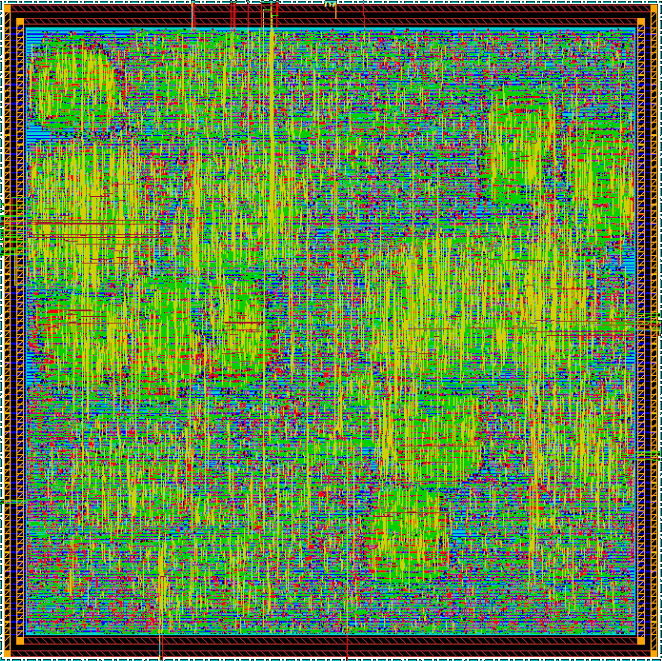
\includegraphics[width=.7\columnwidth]{fpga.png}
	\caption{ASIC Hardware Design of the algorithm implementation on the FPGA}
	\label{fig:fpga}
\end{figure}

\subsection{Pre-processor Circuit Board Design}
Since we aim to utilize our algorithm for pacemakers,
we wanted to make sure that our implementation on the
FPGA could interface with real analog signals. In order
to do this, we designed a preprocessor board that is
capable of sensing electrical activity directly from a
heart and cleaning the signal so that it can properly be
digitized and utilized by the algorithm implementation
on the FPGA. A design drawing of our board, which
utilizes many of the circuit design ideas used in~\cite{analog-adcs}
can be seen in \figurename~\ref{fig:schematic}.

\begin{figure}[h]
	\centering
	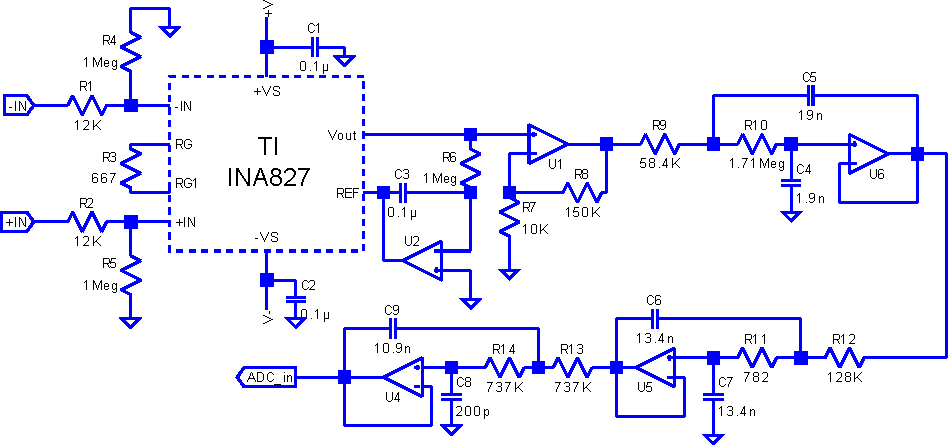
\includegraphics[width=.9\columnwidth]{schematic.pdf}
	\caption{Schematic for preprocessor circuit that senses and cleans analog data from the heart}
	\label{fig:schematic}
\end{figure}

The preprocessor consists of an instrumentation
amplifier, followed by a DC offset removal op-amp, a
non-inverting amplifier, and a 3 stage low pass filter
before going into the logic controller for algorithm
processing. The TI INA827 chip is an instrumentation
amplifier that can take a differential signal as input,
combines it to a single output, and amplifies the signal
by 5. The op amp that feeds back to pin 6 is used to
remove any DC offset or wandering baseline that exists
in the signal. After this stage, the non-inverting amplifier
amplifies the output of the instrumentation amplifier by
16. Finally, there is a 3 stage low pass filter that has a
cutoff frequency at 150 Hz and a gain smaller than -40dB 
starting at 300 Hz. All the chips and op amps are
powered with a +/- 3.3 rail voltage.

\section{Testing and Results}
We validate our ventricular and atrial parameter
learning algorithm and our overarching hardware system
with two separate experiments. The following sections
will describe both tests separately.

\subsection{Ventricular and Atrial Parameter Learning Validation}
In Sections II and III of this paper, we presented an
algorithm that learns \APW{}, \VPW{}, \APH{}, and \VPH{} by
simply processing 10 seconds of CES data sampled at 1
kHz. To validate our solution, we implemented our algorithms in
Matlab and performed atrial and ventricular beat
detection using algorithmically learned parameters on
data provided by the Electrophysiology lab at the Texas Heart Institute.
In order to record the data, an in vivo,
live animal study procedure was performed. For a single
animal, 17 bipolar electrodes populated the left ventricle
of the heart. Each electrode sensed electrical activity
directly from the heart for one minute, digitized the
signal at a 1 kHz sampling rate, and stored the signal as
a .csv file. This was done for 3 animals, giving us a total
of 51 channels that directly resembles the kind of analog
signals a real pacemaker would be sensing.

We then applied our algorithm to data
from each of the 51 channels separately in order to learn
\APW{}, \VPW{}, \APH{}, and \VPH{} specifically for each
channel. Next, using the peak detection algorithm
described in Section III: C, we performed atrial and
ventricular peak detection on each of the 51 channels
using the aforementioned parameters that we computed
for each specific channel. Finally, we computed the
atrial and ventricular beat detection error rate through
tracking false positives (a beat is detected when none
exist) and false negatives (no beat is detected when one
exists) across all 51 channels.
Table~\ref{tab:errors} illustrates our results.
\begin{table}[h]
	\caption{Detection Error Rates using Learned Parameters}
	\label{tab:errors}
	\centering
	\begin{tabular}{|c|c|c|}
		\hline
		Type & False Positive Error Rate & False Negative Error Rate \\
		\hline 
		Ventricles & 0.16\% &4.77\% \\
		\hline
		Atria & 0.89\% & 4.59\% \\
		\hline
		Total & 0.50\% & 4.70 \% \\
		\hline
	\end{tabular}
\end{table}

Our detection error rates are appropriately low across
all 51 channels. Since we performed atrial and
ventricular beat detection based on the parameters that
our algorithm learned, the algorithm clearly learned
\APW{}, \VPW{}, \APH{}, and \VPH{} correctly for the vast
majority of channels. In fact, most of the false negative
error rate results from our algorithm learning incorrect
atrial parameters for one channel. When we manually
looked at the values of \APW{}, \VPW{}, \APH{}, and \VPH{}, we
found that the algorithm learned \VPW{} and \VPH{} correctly
for all 51 channels and \APW{} and \APH{} correctly for 50 of
the channels.

\subsection{Hardware Implementation Validation through a Langendorff Heart}
In order to validate the hardware implementation of
our algorithm described in Section IV, we interfaced our
system to a Langendorff Heart as described by~\cite{langendorff}.
Essentially, in a Langendorff Heart experiment, a live
heart is extracted from a mammal, which in our case was
a rat, and is kept beating. This externally beating heart
will behave as if it was beating internally, so the
Langendroff Heart will retain all of the appropriate
electrical characteristics.
We connected our preprocessor through simple wires
sutured to the Langendroff heart, and then used our
FPGA to digitize the analog signal sensed through the
preprocessor. Our system correctly sensed signals using
the preprocessor, learned pacing parameters (\VPW{} and
\VPH{}), and detected ventricular beats using the learned
values of \VPW{} and \VPH{} in real time. Due to the
relatively small size of a rat's heart in comparison to a
human's, the atrial part of the signal was not
distinguishable on the sensed signal itself, so our
algorithm did not learn any parameters for it.

\section{Conclusions and Future Direction}
We have demonstrated a working algorithm
implemented on hardware that correctly learns \APH{},
\VPH{}, \APW{}, and \VPW{}. Additionally, these parameters
can be reliably used to distinguish between atrial and
ventricular beats in an CES in real time. Future
work will involve utilizing the FPGA implementation of
the algorithm to tape out an application specific
integrated circuit that could be physically placed inside
of a pacemaker.

% An example of a floating figure using the graphicx package.
% Note that \label must occur AFTER (or within) \caption.
% For figures, \caption should occur after the \includegraphics.
% Note that IEEEtran v1.7 and later has special internal code that
% is designed to preserve the operation of \label within \caption
% even when the captionsoff option is in effect. However, because
% of issues like this, it may be the safest practice to put all your
% \label just after \caption rather than within \caption{}.
%
% Reminder: the "draftcls" or "draftclsnofoot", not "draft", class
% option should be used if it is desired that the figures are to be
% displayed while in draft mode.
%
%\begin{figure}[!t]
%\centering
%\includegraphics[width=2.5in]{myfigure}
% where an .eps filename suffix will be assumed under latex, 
% and a .pdf suffix will be assumed for pdflatex; or what has been declared
% via \DeclareGraphicsExtensions.
%\caption{Simulation results for the network.}
%\label{fig_sim}
%\end{figure}

% Note that the IEEE typically puts floats only at the top, even when this
% results in a large percentage of a column being occupied by floats.


% An example of a double column floating figure using two subfigures.
% (The subfig.sty package must be loaded for this to work.)
% The subfigure \label commands are set within each subfloat command,
% and the \label for the overall figure must come after \caption.
% \hfil is used as a separator to get equal spacing.
% Watch out that the combined width of all the subfigures on a 
% line do not exceed the text width or a line break will occur.
%
%\begin{figure*}[!t]
%\centering
%\subfloat[Case I]{\includegraphics[width=2.5in]{box}%
%\label{fig_first_case}}
%\hfil
%\subfloat[Case II]{\includegraphics[width=2.5in]{box}%
%\label{fig_second_case}}
%\caption{Simulation results for the network.}
%\label{fig_sim}
%\end{figure*}
%
% Note that often IEEE papers with subfigures do not employ subfigure
% captions (using the optional argument to \subfloat[]), but instead will
% reference/describe all of them (a), (b), etc., within the main caption.
% Be aware that for subfig.sty to generate the (a), (b), etc., subfigure
% labels, the optional argument to \subfloat must be present. If a
% subcaption is not desired, just leave its contents blank,
% e.g., \subfloat[].


% An example of a floating table. Note that, for IEEE style tables, the
% \caption command should come BEFORE the table and, given that table
% captions serve much like titles, are usually capitalized except for words
% such as a, an, and, as, at, but, by, for, in, nor, of, on, or, the, to
% and up, which are usually not capitalized unless they are the first or
% last word of the caption. Table text will default to \footnotesize as
% the IEEE normally uses this smaller font for tables.
% The \label must come after \caption as always.
%
%\begin{table}[!t]
%% increase table row spacing, adjust to taste
%\renewcommand{\arraystretch}{1.3}
% if using array.sty, it might be a good idea to tweak the value of
% \extrarowheight as needed to properly center the text within the cells
%\caption{An Example of a Table}
%\label{table_example}
%\centering
%% Some packages, such as MDW tools, offer better commands for making tables
%% than the plain LaTeX2e tabular which is used here.
%\begin{tabular}{|c||c|}
%\hline
%One & Two\\
%\hline
%Three & Four\\
%\hline
%\end{tabular}
%\end{table}


% Note that the IEEE does not put floats in the very first column
% - or typically anywhere on the first page for that matter. Also,
% in-text middle ("here") positioning is typically not used, but it
% is allowed and encouraged for Computer Society conferences (but
% not Computer Society journals). Most IEEE journals/conferences use
% top floats exclusively. 
% Note that, LaTeX2e, unlike IEEE journals/conferences, places
% footnotes above bottom floats. This can be corrected via the
% \fnbelowfloat command of the stfloats package.




% trigger a \newpage just before the given reference
% number - used to balance the columns on the last page
% adjust value as needed - may need to be readjusted if
% the document is modified later
%\IEEEtriggeratref{8}
% The "triggered" command can be changed if desired:
%\IEEEtriggercmd{\enlargethispage{-5in}}

% references section

% can use a bibliography generated by BibTeX as a .bbl file
% BibTeX documentation can be easily obtained at:
% http://mirror.ctan.org/biblio/bibtex/contrib/doc/
% The IEEEtran BibTeX style support page is at:
% http://www.michaelshell.org/tex/ieeetran/bibtex/
\bibliographystyle{IEEEtran}
% argument is your BibTeX string definitions and bibliography database(s)
\bibliography{IEEEabrv,sources}



% that's all folks
\end{document}


